\section{Hardware Design} \label{sec:hard-design}

\onehalfspacing

\subsection{Goals}

The smart containers that will house emergency medical devices are meant to resemble existing Automated Emergency Defibrillator (AED) units that are currently in use. This existing type of container is well-known in most communities and will serve as a familiar interface for users when using the new containers. The new, smart containers (henceforth referred to as ``containers'') are designed to perform a variety of functions to assist users who are trying to locate an emergency medical device. For purposes of discussion, we will assume that the containers will house both autoinjectors and defibrillators. In the following sections, we discuss the features and design choices of the smart container.

\subsection{Form Factor}

Current AED defibrillator containers come in a variety of sizes and models depending on how the container is mounted to the wall, but the interior of most boxes measures around 12$''$ $\times$ 12$''$ $\times$ 5$''$, with the defibrillators themselves measuring around 8$''$ $\times$ 6$''$ $\times$ 3$''$. We will assume that the autoinjectors we store in the containers are the same size as those purchased with a prescription (approximately 5$''$ $\times$ 1$''$ $\times$ 1$''$), but in practice it might be prudent to create a larger autoinjector form factor that would be harder to steal from the container. Current AED defibrillator containers store one defibrillator per container, and we will do the same. We will also store two autoinjectors per container, as most autoinjector manufacturers recommend carrying two at all times in case one should fail.

Besides simply storing the medical devices, we also wish to assist users who are looking for the containers and make it as easy as possible to locate. Instead of only providing the location of a container through the mobile app, we also use physical light and sound signals on a container to help direct users to the correct location. The container will feature LED lights that will flash and speakers that will make noise when a user is looking for a container. In addition to these signals, a touch screen will also provide a user interface that will allow users to control the lights and sounds of the box. Furthermore, a screen could be used to show the location of a user who is looking for the container, allowing people nearby to assist in getting the necessary medical devices to the use in need. Because the epinephrine used in autoinjectors is sensitive to temperature changes and must be kept within a specified temperature range, we use a discrete temperature sensor inside the container to monitor the containers temperature an ensure that these temperature requirements are not broken.

In order to facilitate the communication between the container and the server, we use an Internet-connected microcontroller ($\mu$C) and a network controller. These will be discretely located within the container and used to control the peripherals based on messages received from the server and commands received from the user-facing touch screen.

\subsection{Electronics}

The circuitry consists of five main components:
\begin{enumerate}
    \item Microcontroller
    \item Touch screen
    \item Temperature, humidity, and air pressure sensors
    \item Lights
    \item Speakers
\end{enumerate}

The microcontroller selected was the Atmel ATSAMD21G18. This chip has 256 kB of flash, 32 kB of SRAM, 6 serial communication modules, and 20 output pins. This is enough memory and I/O capability to allow for multiple peripherals, including the touch screen, temperature sensor, LEDs, and speakers while remaining comparatively inexpensive. The network controller selected was the Atmel ATWINC1500, an IEEE 802.11 b/g/n WiFi chip with a single-band 2.3 GHz channel that supports WPA/WPA2 Personal and SSL security protocols. The Adafruit Arduino Feather M0 was selected as the breakout board for prototyping and contains both the ATSAMD21G18 and ATWINC1500 chips. The Arduino IDE and bootloader were used for programming the microcontroller.

The touch screen used for the container was the Adafruit 2.8$''$ TFT LCD Touchscreen Breakout Board. This board is capable of simple SPI communication and allows for minimal microcontroller pin usage. The board is also has a self-contained controller, so minimal graphic computations are required on the main microcontroller. This screen is small compared to most mobile phone touch screens but is large enough to provide a simple user interface for controlling the container.

The temperature sensor selected was the Bosch BME280, an environmental sensor that measures temperature, humidity, and air pressure with $\pm$ 1.0\degree C, $\pm$ 3\%, and $\pm$ 1 hPa accuracies respectively. When measuring only temperature and humidity, it draws only 1.8 $\mu$A of current, dissipating 5.94 $\mu$W of power when used with 3.3 V logic. For lighting, an iPixel APA102 addressable 1m LED light strip was selected. This allows for unique light patterns to be generated by the microcontroller that can be used to direct users to the container. Two, 3$''$ 4 $\ohm$ 3 W speakers were used for sound signals. 

\begin{figure}
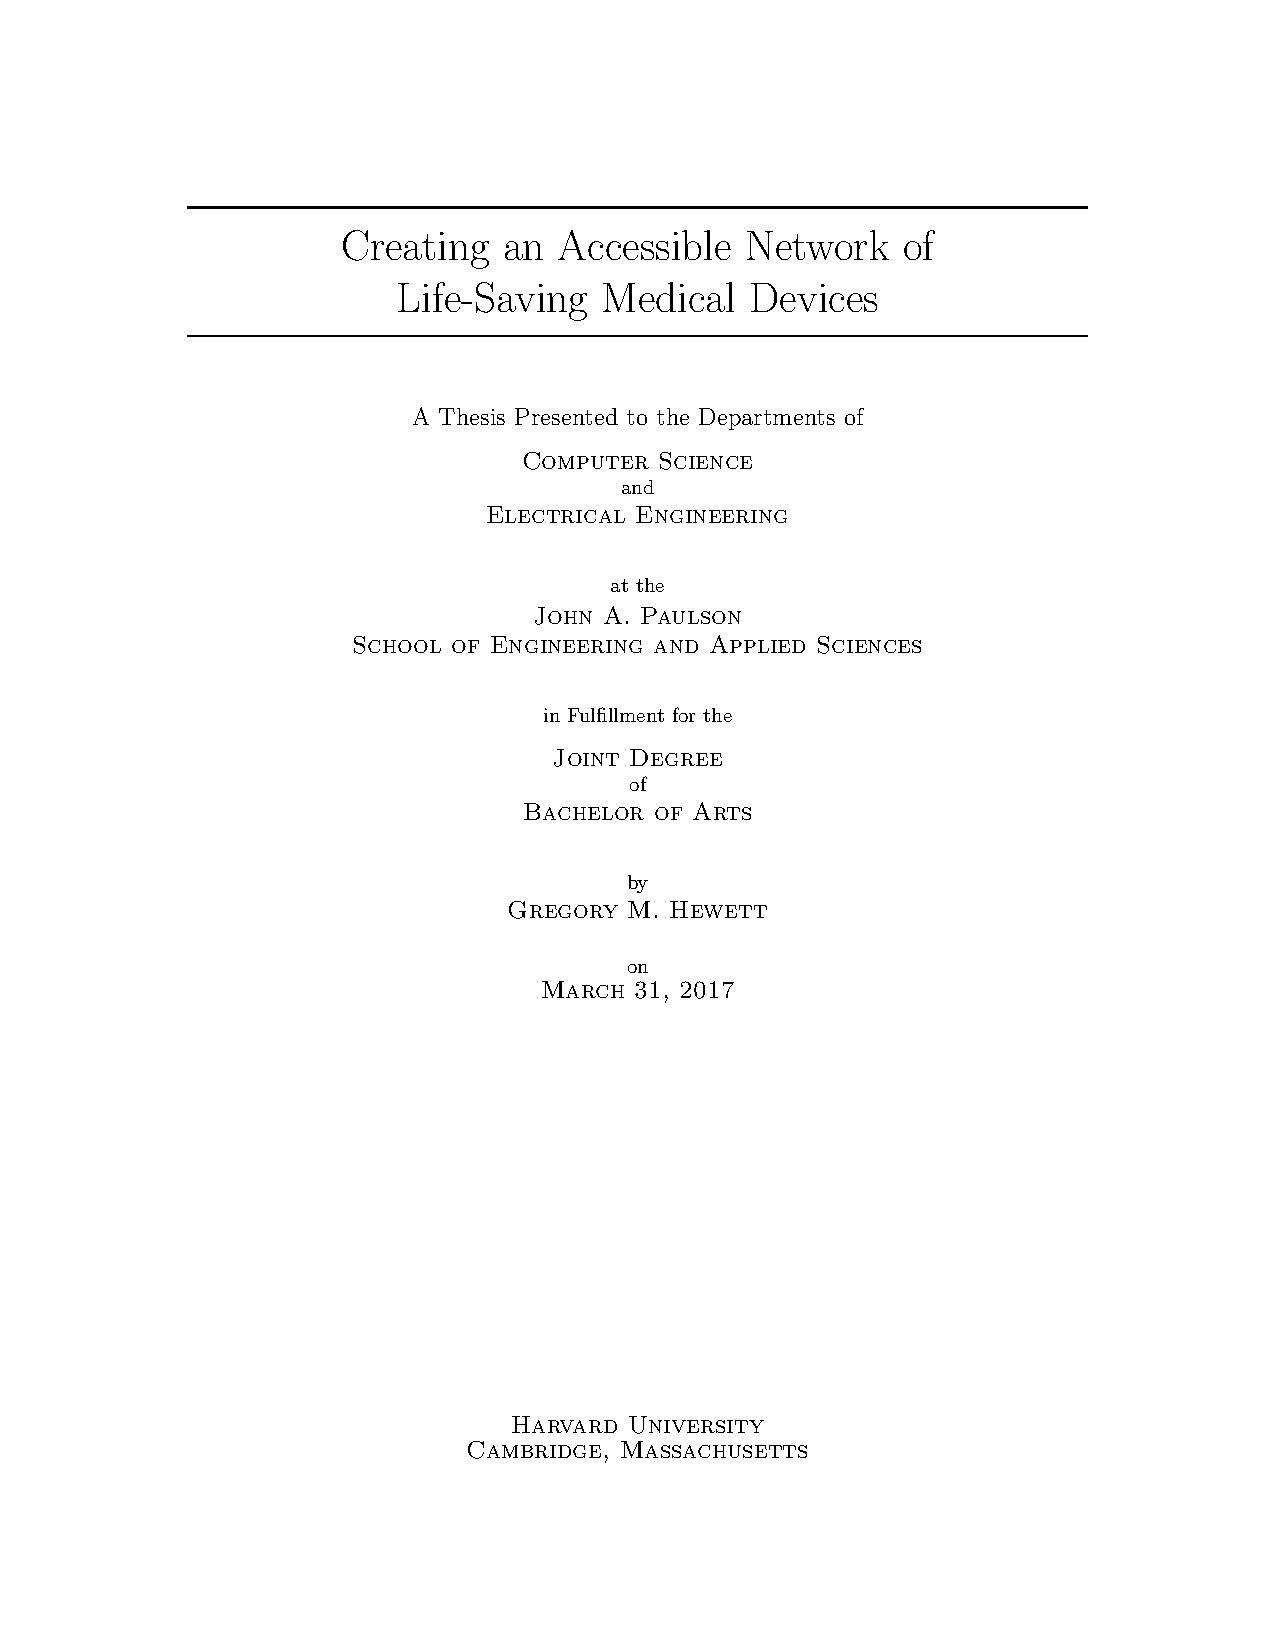
\includegraphics[width=\linewidth]{main}
\caption{Main schematic.}
\label{fig:mainschem}
\end{figure}

\subsection{Network Protocols}











